\documentclass[12pt,letterpaper]{article}
\usepackage{graphicx,textcomp}
\usepackage{natbib}
\usepackage{setspace}
\usepackage{fullpage}
\usepackage{color}
\usepackage[reqno]{amsmath}
\usepackage{amsthm}
\usepackage{fancyvrb}
\usepackage{amssymb,enumerate}
\usepackage[all]{xy}
\usepackage{endnotes}
\usepackage{lscape}
\newtheorem{com}{Comment}
\usepackage{float}
\usepackage{hyperref}
\newtheorem{lem} {Lemma}
\newtheorem{prop}{Proposition}
\newtheorem{thm}{Theorem}
\newtheorem{defn}{Definition}
\newtheorem{cor}{Corollary}
\newtheorem{obs}{Observation}
\usepackage[compact]{titlesec}
\usepackage{dcolumn}
\usepackage{tikz}
\usetikzlibrary{arrows}
\usepackage{multirow}
\usepackage{xcolor}
\newcolumntype{.}{D{.}{.}{-1}}
\newcolumntype{d}[1]{D{.}{.}{#1}}
\definecolor{light-gray}{gray}{0.65}
\usepackage{url}
\usepackage{listings}
\usepackage{color}

\definecolor{codegreen}{rgb}{0,0.6,0}
\definecolor{codegray}{rgb}{0.5,0.5,0.5}
\definecolor{codepurple}{rgb}{0.58,0,0.82}
\definecolor{backcolour}{rgb}{0.95,0.95,0.92}

\lstdefinestyle{mystyle}{
	backgroundcolor=\color{backcolour},   
	commentstyle=\color{codegreen},
	keywordstyle=\color{magenta},
	numberstyle=\tiny\color{codegray},
	stringstyle=\color{codepurple},
	basicstyle=\footnotesize,
	breakatwhitespace=false,         
	breaklines=true,                 
	captionpos=b,                    
	keepspaces=true,                 
	numbers=left,                    
	numbersep=5pt,                  
	showspaces=false,                
	showstringspaces=false,
	showtabs=false,                  
	tabsize=2
}
\lstset{style=mystyle}
\newcommand{\Sref}[1]{Section~\ref{#1}}
\newtheorem{hyp}{Hypothesis}

\title{Problem Set 1}
\date{Due: September 30, 2024}
\author{Applied Stats/Quant Methods 1}

\begin{document}
	\maketitle
	
	\section*{Instructions}
	\begin{itemize}
	\item Please show your work! You may lose points by simply writing in the answer. If the problem requires you to execute commands in \texttt{R}, please include the code you used to get your answers. Please also include the \texttt{.R} file that contains your code. If you are not sure if work needs to be shown for a particular problem, please ask.
\item Your homework should be submitted electronically on GitHub.
\item This problem set is due before 23:59 on Monday September 30, 2024. No late assignments will be accepted.
%\item Total available points for this homework is 80.
	\end{itemize}
	
	\vspace{1cm}
	\section*{Question 1: Education}

A school counselor was curious about the average of IQ of the students in her school and took a random sample of 25 students' IQ scores. The following is the data set:\\
\vspace{.5cm}

\lstinputlisting[language=R, firstline=36, lastline=36]{my_answers_RJ.C.R}  

\vspace{1cm}

\begin{enumerate}
	\item Find a 90\% confidence interval for the average student IQ in the school.\\
	\lstinputlisting[language=R, firstline=47, lastline=54]{my_answersRJ.C.R}
	\begin{verbatim}
		Confidence interval (93.95993 102.92007) mean value(98.44000)
	\end{verbatim} 
	\item Next, the school counselor was curious  whether  the average student IQ in her school is higher than the average IQ score (100) among all the schools in the country.\\ 
	\noindent Using the same sample, conduct the appropriate hypothesis test with $\alpha=0.05$.

	\lstinputlisting[language=R, firstline=55, lastline=76]{my_answersRJ.C.R}  
\end{enumerate}

\newpage

	\section*{Question 2: Political Economy}

\noindent Researchers are curious about what affects the amount of money communities spend on addressing homelessness. The following variables constitute our data set about social welfare expenditures in the USA. \\
\vspace{.5cm}


\begin{tabular}{r|l}
	\texttt{State} &\emph{50 states in US} \\
	\texttt{Y} & \emph{per capita expenditure on shelters/housing assistance in state}\\
	\texttt{X1} &\emph{per capita personal income in state} \\
	\texttt{X2} &  \emph{Number of residents per 100,000 that are "financially insecure" in state}\\
	\texttt{X3} &  \emph{Number of people per thousand residing in urban areas in state} \\
	\texttt{Region} &  \emph{1=Northeast, 2= North Central, 3= South, 4=West} \\
\end{tabular}

\vspace{.5cm}
\noindent Explore the \texttt{expenditure} data set and import data into \texttt{R}.
\vspace{.5cm}
\lstinputlisting[language=R, firstline=54, lastline=54]{my_answers_RJ.C.R}  
\vspace{.5cm}
\begin{itemize}

\item
Please plot the relationships among \emph{Y}, \emph{X1}, \emph{X2}, and \emph{X3}? What are the correlations among them (you just need to describe the graph and the relationships among them)?

\lstinputlisting[language=R, firstline=116, lastline=116]{my_answersRJ.C.R}
    \begin{enumerate}
	\item[]
	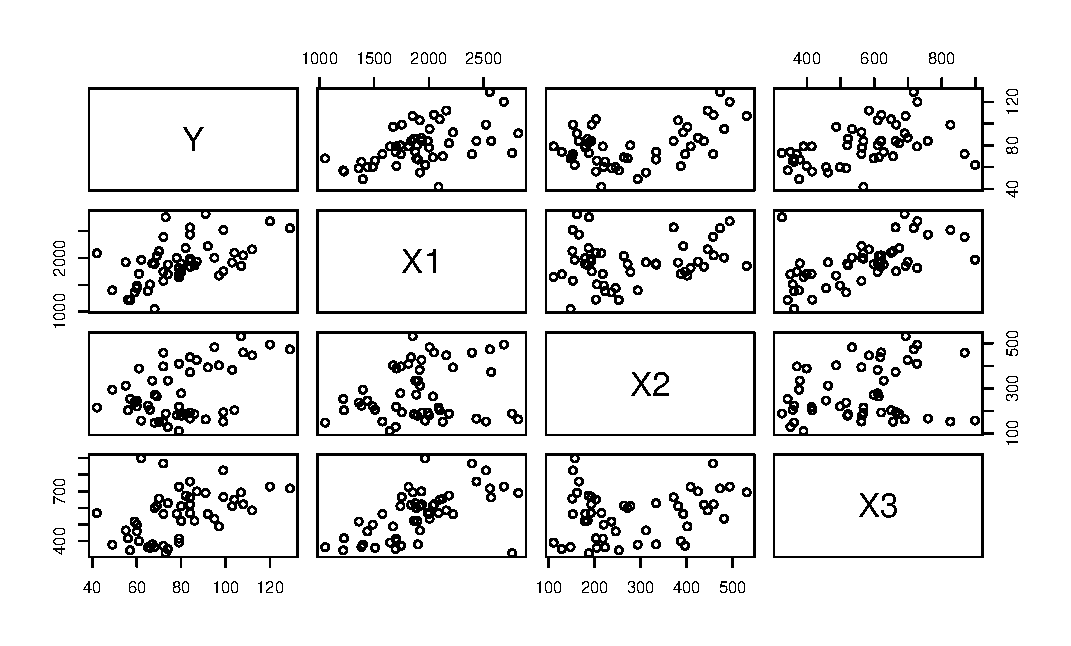
\includegraphics[width=.85\textwidth]{plot.all relationship_RJ.C.pdf}
   \end{enumerate}
\lstinputlisting[language=R, firstline=119, lastline=119]{my_answersRJ.C.R}
	\begin{verbatim}
	  STATE                 Y                X1             X2              X3       
	Length:50          Min.   : 42.00   Min.   :1053   Min.   :111.0   Min.   :326.0  
	Class :character   1st Qu.: 67.25   1st Qu.:1698   1st Qu.:187.2   1st Qu.:426.2  
	Mode  :character   Median : 79.00   Median :1897   Median :241.5   Median :568.0  
	                   Mean   : 79.54   Mean   :1912   Mean   :281.8   Mean   :561.7  
	                   3rd Qu.: 90.00   3rd Qu.:2096   3rd Qu.:391.8   3rd Qu.:661.2  
	                   Max.   :129.00   Max.   :2817   Max.   :531.0   Max.   :899.0 
  \end{verbatim} 
\lstinputlisting[language=R, firstline=145, lastline=147]{my_answersRJ.C.R}
  \begin{enumerate}
  	\item[]
  	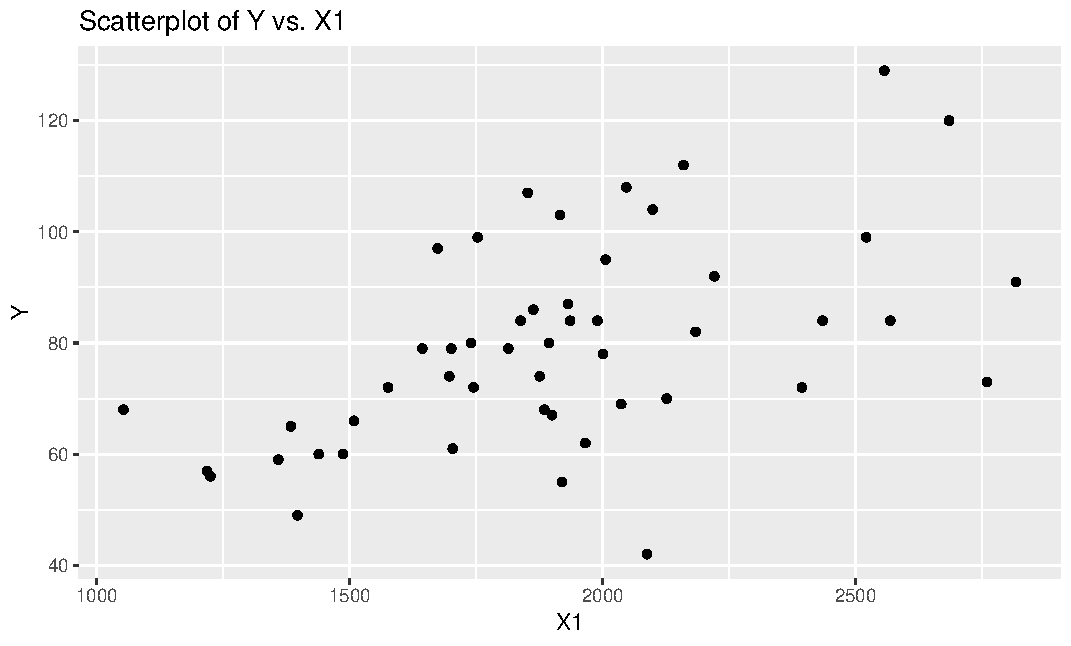
\includegraphics[width=.80\textwidth]{plot.Y.X1_RJ.C.pdf}
  \end{enumerate}
  \begin{verbatim}
  	Y is positively correlated with x1,
  	 indicating that as personal income increases, 
  	 per capita housing expenditure also increases
  \end{verbatim} 
\lstinputlisting[language=R, firstline=155, lastline=155]{my_answersRJ.C.R}
  %  \begin{table}[htbp]
  %		\centering
  %		\caption{}  
  %	    \label{}
  %		
===============================================
                        Dependent variable:    
                    ---------------------------
                                 Y             
-----------------------------------------------
X1                           0.025***          
                              (0.006)          
                                               
Constant                     32.546***         
                             (11.034)          
                                               
-----------------------------------------------
Observations                    50             
R2                             0.283           
Adjusted R2                    0.268           
Residual Std. Error      15.836 (df = 48)      
F Statistic           18.920*** (df = 1; 48)   
===============================================
Note:               *p<0.1; **p<0.05; ***p<0.01

  %	  \end{table}
  %  problem:The format in the file is correct, but when imported into LaTeX, the format changes
  \begin{table}[!htbp] \centering 
  	\caption{} 
  	\label{} 
  	\begin{tabular}{@{\extracolsep{5pt}}lc} 
  		\\[-2.8ex]\hline 
  		\hline \\[-2.8ex] 
  		& \multicolumn{1}{c}{\textit{Dependent variable:}} \\ 
  		\cline{2-2} 
  		\\[-2.8ex] & Y \\ 
  		\hline \\[-2.8ex] 
  		X1 & 0.025$^{***}$ \\ 
  		& (0.006) \\ 
  		& \\ 
  		Constant & 32.546$^{***}$ \\ 
  		& (11.034) \\ 
  		& \\ 
  		\hline \\[-2.8ex] 
  		Observations & 50 \\ 
  		R$^{2}$ & 0.283 \\ 
  		Adjusted R$^{2}$ & 0.268 \\ 
  		Residual Std. Error & 15.836 (df = 48) \\ 
  		F Statistic & 18.920$^{***}$ (df = 1; 48) \\ 
  		\hline 
  		\hline \\[-2.8ex] 
  		\textit{Note:}  & \multicolumn{1}{r}{$^{*}$p$<$0.1; $^{**}$p$<$0.05; $^{***}$p$<$0.01} \\ 
  	\end{tabular} 
  \end{table} 
\vspace{2.5cm} 
\begin{verbatim}
	The coefficient of X1 is 0.025 and has statistical significance (p-value<0.01), 
	indicating a positive correlation between X1 and Y. 
	Specifically, for every unit increase in X1, Y is expected to increase by 0.025 units; 
	The constant term is 32.546 and has statistical significance (p-value<0.01). 
	This means that when X1 is zero, the expected value of Y is 32.546; 
	The adjusted R-squared is 0.268, slightly lower than R-squared,
	indicating that there are other factors affecting housing expenditure;
	as per capita income (X1) increases, housing expenditure (Y) will also increase
\end{verbatim}
  %Y与X1
\vspace{5.5cm}
\lstinputlisting[language=R, firstline=174, lastline=176]{my_answersRJ.C.R}
\begin{enumerate}
	\item[]
	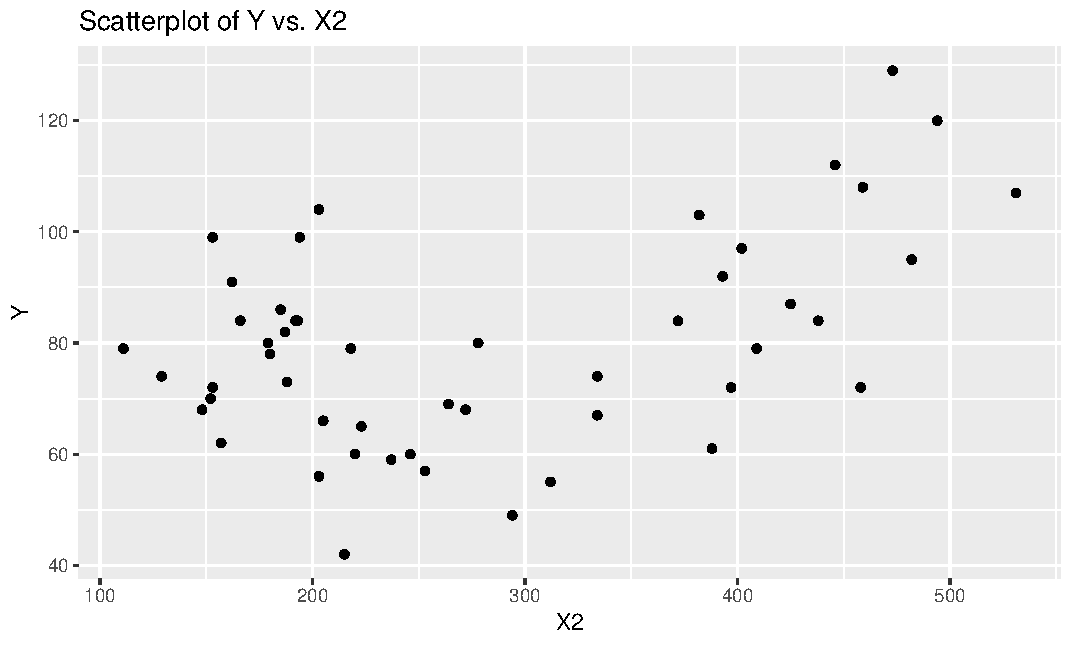
\includegraphics[width=.80\textwidth]{plot.Y.X2_RJ.C.pdf}
\end{enumerate}
\begin{verbatim}
	There is a positive correlation between y and x2, 
	indicating that in continents with more economically unstable residents,
	per capita housing expenditures will increase
\end{verbatim}
\lstinputlisting[language=R, firstline=185, lastline=185]{my_answersRJ.C.R}
\begin{table}[!htbp] \centering 
	\caption{} 
	\label{} 
	\begin{tabular}{@{\extracolsep{5pt}}lc} 
		\\[-2.8ex]\hline 
		\hline \\[-2.8ex] 
		& \multicolumn{1}{c}{\textit{Dependent variable:}} \\ 
		\cline{2-2} 
		\\[-2.8ex] & Y \\ 
		\hline \\[-2.8ex] 
		X2 & 0.070$^{***}$ \\ 
		& (0.020) \\ 
		& \\ 
		Constant & 57.761$^{***}$ \\ 
		& (6.164) \\ 
		& \\ 
		\hline \\[-2.8ex] 
		Observations & 50 \\ 
		R$^{2}$ & 0.201 \\ 
		Adjusted R$^{2}$ & 0.184 \\ 
		Residual Std. Error & 16.714 (df = 48) \\ 
		F Statistic & 12.072$^{***}$ (df = 1; 48) \\ 
		\hline 
		\hline \\[-2.8ex] 
		\textit{Note:}  & \multicolumn{1}{r}{$^{*}$p$<$0.1; $^{**}$p$<$0.05; $^{***}$p$<$0.01} \\ 
	\end{tabular} 
\end{table}  
\begin{verbatim}
	The coefficient of X2 is 0.070 and has statistical significance (p-value<0.01), 
	indicating a positive correlation between X2 and Y; 
	The R-squared value is 0.201, indicating that X2 can explain 20.1% of Y variability 
	and suggesting that there are other factors affecting Y
\end{verbatim}
%Y与X2

\lstinputlisting[language=R, firstline=192, lastline=194]{my_answersRJ.C.R}
\begin{enumerate}
	\item[]
	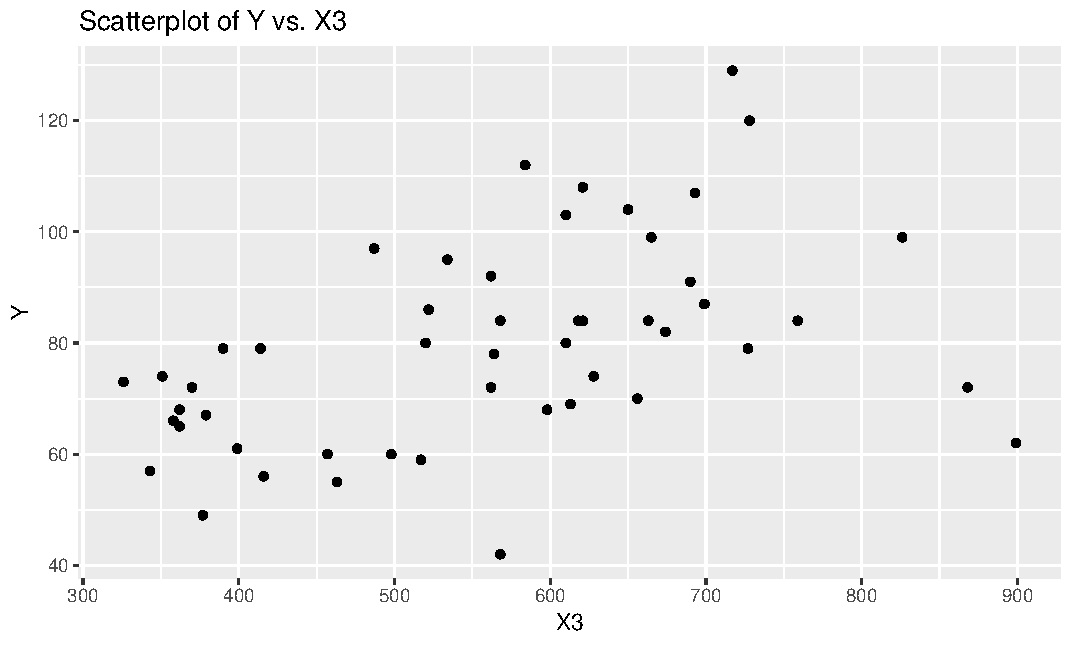
\includegraphics[width=.75\textwidth]{plot.Y.X3_RJ.C.pdf}
\end{enumerate}
\begin{verbatim}
	There is a positive correlation between y and x3, 
	indicating that in continents with higher urbanization, 
	per capita housing expenditures will also increase
\end{verbatim}
\lstinputlisting[language=R, firstline=203, lastline=203]{my_answersRJ.C.R}
\begin{table}[!htbp] \centering 
	\caption{} 
	\label{} 
	\begin{tabular}{@{\extracolsep{5pt}}lc} 
		\\[-2.8ex]\hline 
		\hline \\[-1.8ex] 
		& \multicolumn{1}{c}{\textit{Dependent variable:}} \\ 
		\cline{2-2} 
		\\[-2.8ex] & Y \\ 
		\hline \\[-2.8ex] 
		X3 & 0.059$^{***}$ \\ 
		& (0.016) \\ 
		& \\ 
		Constant & 43.306$^{***}$ \\ 
		& (9.461) \\ 
		& \\ 
		\hline \\[-2.8ex] 
		Observations & 50 \\ 
		R$^{2}$ & 0.215 \\ 
		Adjusted R$^{2}$ & 0.199 \\ 
		Residual Std. Error & 16.567 (df = 48) \\ 
		F Statistic & 13.1146$^{***}$ (df = 1; 48) \\ 
		\hline 
		\hline \\[-2.8ex] 
		\textit{Note:}  & \multicolumn{1}{r}{$^{*}$p$<$0.1; $^{**}$p$<$0.05; $^{***}$p$<$0.01} \\ 
	\end{tabular}
\end{table}     
\begin{verbatim}
The coefficient of X3 is 0.059 and has statistical significance (p-value<0.01), 
indicating a positive correlation between X3 and Y; 
The R-squared value is 0.215, indicating that X3 can explain 21.5% of Y variability. 
This is a relatively low value, 
indicating that there are other factors affecting Y
\end{verbatim}
%Y与X3
\vspace{10.5cm} 
\lstinputlisting[language=R, firstline=210, lastline=212]{my_answersRJ.C.R}
\begin{enumerate}
	\item[]
	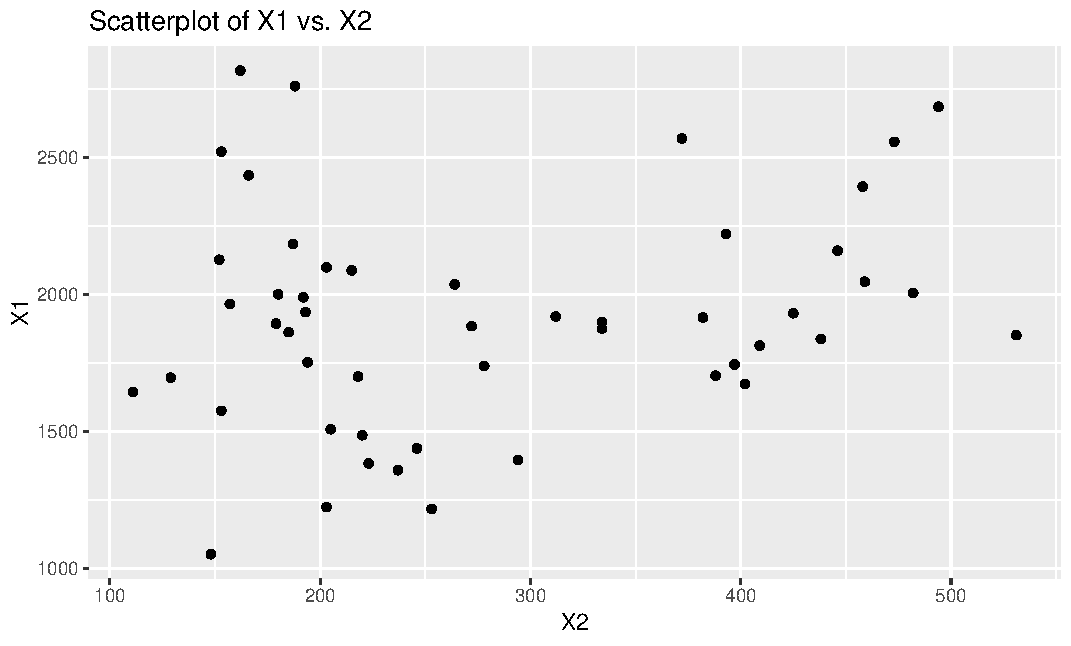
\includegraphics[width=.75\textwidth]{plot.X1.X2_RJ.C.pdf}
\end{enumerate}
\begin{verbatim} 
	There is a negative correlation between x1 and x2. 
	Continents with high per capita income 
	fewer residents with unstable economies
\end{verbatim}
\lstinputlisting[language=R, firstline=221, lastline=221]{my_answersRJ.C.R}
\begin{table}[!htbp] \centering 
	\caption{} 
	\label{} 
	\begin{tabular}{@{\extracolsep{5pt}}lc} 
		\\[-2.8ex]\hline 
		\hline \\[-1.8ex] 
		& \multicolumn{1}{c}{\textit{Dependent variable:}} \\ 
		\cline{2-2} 
		\\[-2.8ex] & X1 \\ 
		\hline \\[-2.8ex] 
		X2 & 0.696$^{***}$ \\ 
		& (0.478) \\ 
		& \\ 
		Constant & 1715.655$^{***}$ \\ 
		& (145.981) \\ 
		& \\ 
		\hline \\[-2.8ex] 
		Observations & 50 \\ 
		R$^{2}$ & 0.042 \\ 
		Adjusted R$^{2}$ & 0.022 \\ 
		Residual Std. Error & 395.854 (df = 48) \\ 
		F Statistic & 2.119$^{***}$ (df = 1; 48) \\ 
		\hline 
		\hline \\[-2.8ex] 
		\textit{Note:}  & \multicolumn{1}{r}{$^{*}$p$<$0.1; $^{**}$p$<$0.05; $^{***}$p$<$0.01} \\ 
	\end{tabular} 
\end{table}  
\begin{verbatim} 
The coefficient of X2 is 0.696, 
but this coefficient is not statistically significant (p-value>0.1),
which means there is not enough evidence to 
conclude a significant linear relationship between X2 and X1; 
The R-squared value is 0.042, indicating that X2 can explain 4.2% of X1's variability. 
This is a very low value, indicating a very weak relationship between X2 and X1
\end{verbatim}
%X1与X2
\vspace{10.5cm} 
\lstinputlisting[language=R, firstline=229, lastline=231]{my_answersRJ.C.R}
\begin{enumerate}
	\item[]
	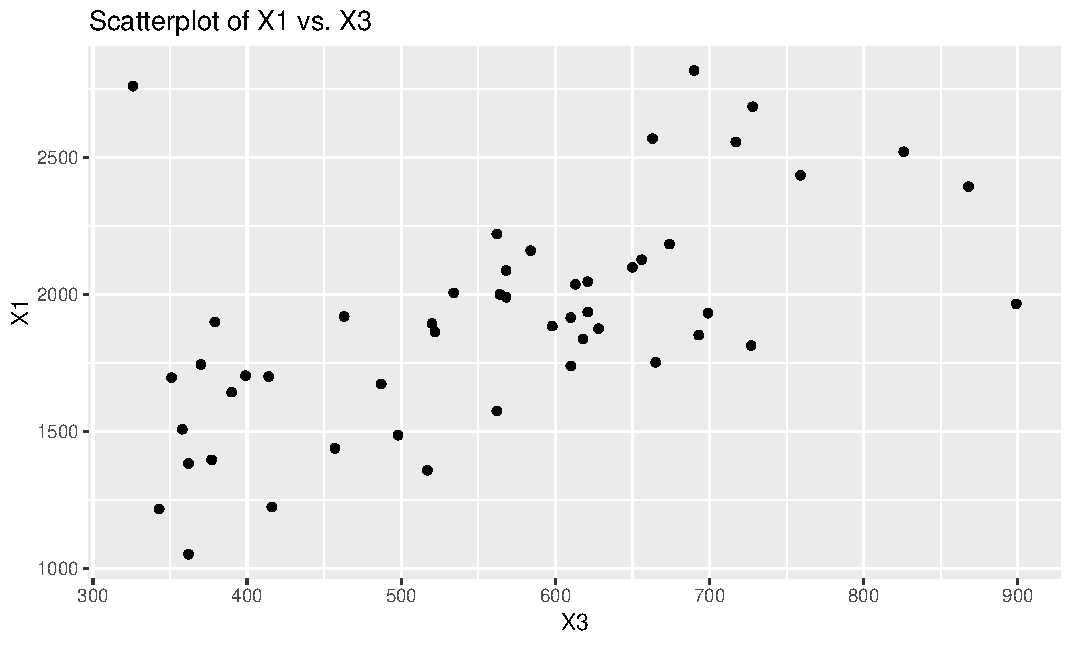
\includegraphics[width=.75\textwidth]{plot.X1.X3_RJ.C.pdf}
\end{enumerate}
\begin{verbatim} 
	There is a positive correlation between x1 and x3, 
	the higher the urbanization of the continent, 
	the higher the per capita income
\end{verbatim}
\lstinputlisting[language=R, firstline=240, lastline=240]{my_answersRJ.C.R}
\begin{table}[!htbp] \centering 
	\caption{} 
	\label{} 
	\begin{tabular}{@{\extracolsep{5pt}}lc} 
		\\[-2.8ex]\hline 
		\hline \\[-1.8ex] 
		& \multicolumn{1}{c}{\textit{Dependent variable:}} \\ 
		\cline{2-2} 
		\\[-2.8ex] & X1 \\ 
		\hline \\[-2.8ex] 
		X3 & 1.643$^{***}$ \\ 
		& (0.320) \\ 
		& \\ 
		Constant & 988.947$^{***}$ \\ 
		& (185.614) \\ 
		& \\ 
		\hline \\[-2.8ex] 
		Observations & 50 \\ 
		R$^{2}$ & 0.354 \\ 
		Adjusted R$^{2}$ & 0.341 \\ 
		Residual Std. Error & 325.029 (df = 48) \\ 
		F Statistic & 26.341$^{***}$ (df = 1; 48) \\ 
		\hline 
		\hline \\[-2.8ex] 
		\textit{Note:}  & \multicolumn{1}{r}{$^{*}$p$<$0.1; $^{**}$p$<$0.05; $^{***}$p$<$0.01} \\ 
	\end{tabular} 
\end{table} 
\begin{verbatim} 
The coefficient of X3 is 1.643 and has statistical significance (p-value<0.01), 
indicating a positive correlation between X3 and X1; 
The R-squared value is 0.354, 
indicating that X3 can explain 35.4% of X1's variability. 
This is a moderate value, 
indicating that X3 has a certain explanatory power for X1
\end{verbatim}
 %X1与X3
\vspace{10.5cm}
\lstinputlisting[language=R, firstline=247, lastline=249]{my_answersRJ.C.R}
\begin{enumerate}
	\item[]
	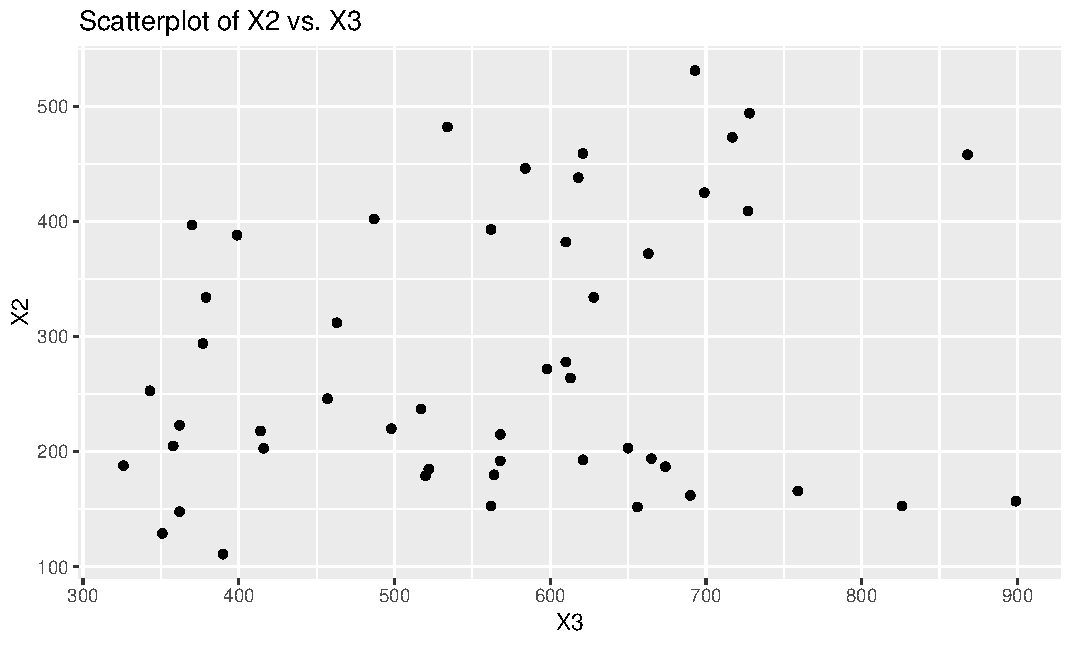
\includegraphics[width=.75\textwidth]{plot.X2.X3_RJ.C.pdf}
\end{enumerate}
	\begin{verbatim} 
	The correlation between X2 and X3 is weak
	the degree of urbanization has little to do with economic instability
\end{verbatim}
\lstinputlisting[language=R, firstline=258, lastline=258]{my_answersRJ.C.R}
\begin{table}[!htbp] \centering 
	\caption{} 
	\label{} 
	\begin{tabular}{@{\extracolsep{5pt}}lc} 
		\\[-2.8ex]\hline 
		\hline \\[-2.8ex] 
		& \multicolumn{1}{c}{\textit{Dependent variable:}} \\ 
		\cline{2-2} 
		\\[-2.8ex] & X2 \\ 
		\hline \\[-2.8ex] 
		X3 & 0.180$^{***}$ \\ 
		& (0.115) \\ 
		& \\ 
		Constant & 180.609$^{***}$ \\ 
		& (66.509) \\ 
		& \\ 
		\hline \\[-2.8ex] 
		Observations & 50 \\ 
		R$^{2}$ & 0.049 \\ 
		Adjusted R$^{2}$ & 0.029 \\ 
		Residual Std. Error & 116.465 (df = 48) \\ 
		F Statistic & 2.465$^{***}$ (df = 1; 48) \\ 
		\hline 
		\hline \\[-2.8ex] 
		\textit{Note:}  & \multicolumn{1}{r}{$^{*}$p$<$0.1; $^{**}$p$<$0.05; $^{***}$p$<$0.01} \\ 
	\end{tabular} 
\end{table} 
\begin{verbatim} 
The coefficient of X3 is 0.180, 
but this coefficient is not statistically significant (p-value>0.1) 
because there is no asterisk mark next to the coefficient, 
which cannot prove a significant linear relationship between X3 and X2; 
The R-squared value is 0.049, 
indicating that X3 can explain 4.9% of X2 variability. 
This is a very low value, 
indicating a very weak relationship between X3 and X2, 
suggesting that there are other important factors affecting X2
\end{verbatim}
 %X2与X3

\vspace{11.5cm}

\item
Please plot the relationship between \emph{Y} and \emph{Region}? On average, which region has the highest per capita expenditure on housing assistance?

\lstinputlisting[language=R, firstline=133, lastline=135]{my_answersRJ.C.R}
   \begin{enumerate}
   	\item[]
  	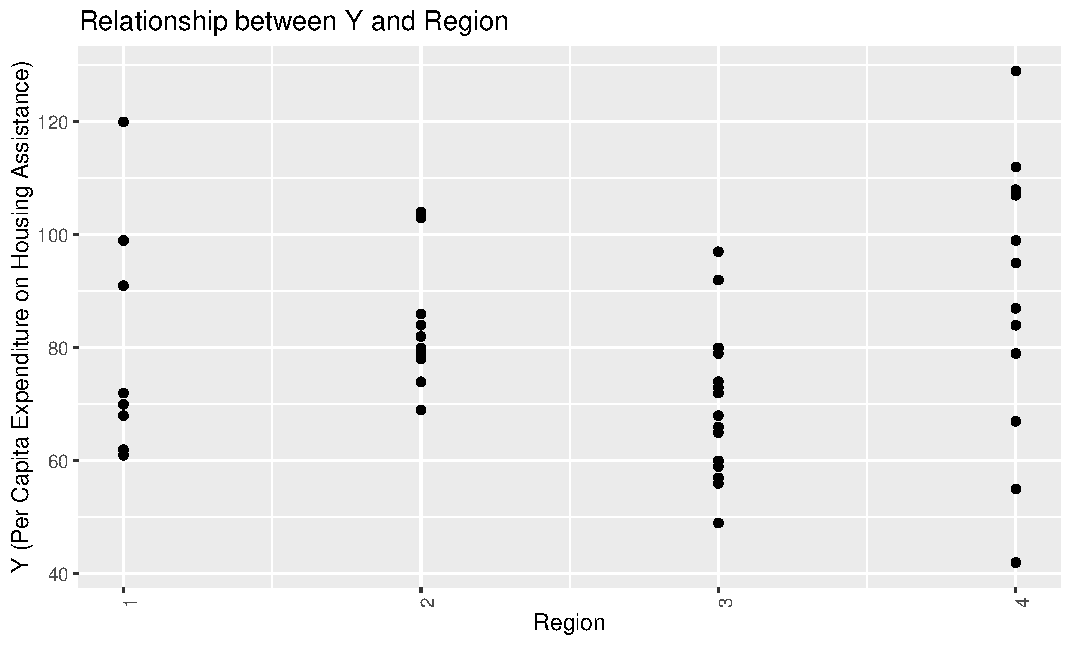
\includegraphics[width=.85\textwidth]{plot.Y.Region_RJ.C.pdf}
   \end{enumerate}
\lstinputlisting[language=R, firstline=137, lastline=138]{my_answersRJ.C.R}
    \begin{verbatim}
    	                  Region        Y
    	                    4        88.30769
    \end{verbatim} 
\vspace{.5cm}
\item
Please plot the relationship between \emph{Y} and \emph{X1}? Describe this graph and the relationship. Reproduce the above graph including one more variable \emph{Region} and display different regions with different types of symbols and colors.

\lstinputlisting[language=R, firstline=145, lastline=147]{my_answersRJ.C.R}
           \begin{enumerate}
           	\item[]
         	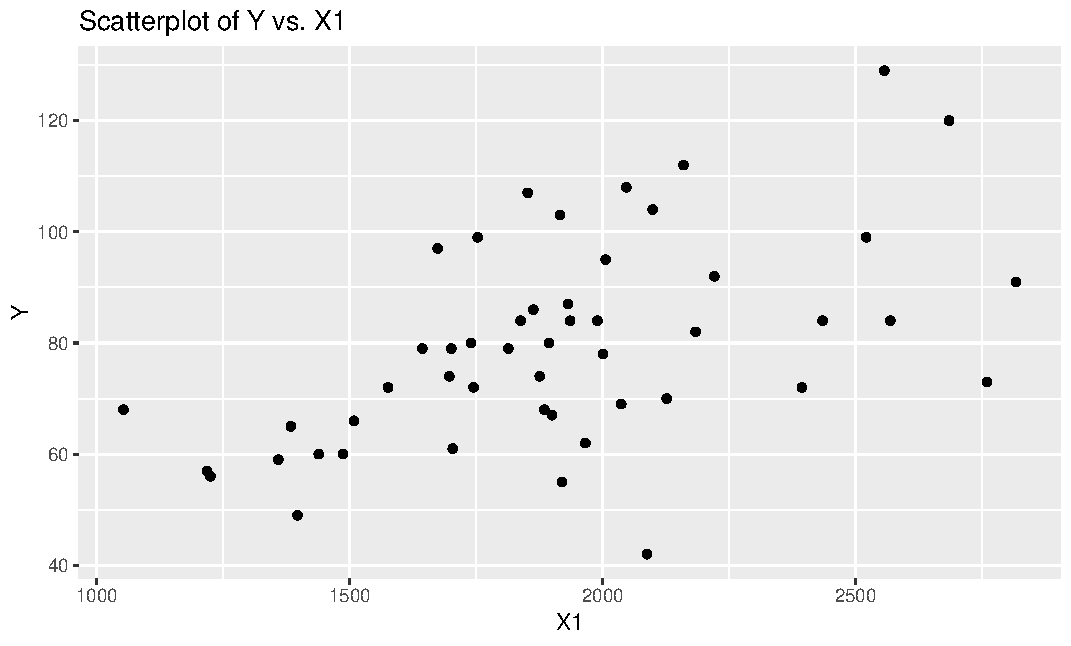
\includegraphics[width=.85\textwidth]{plot.Y.X1_RJ.C.pdf}
           \end{enumerate} 
       \begin{verbatim}
      Y is strongly positively correlated with X1
      as per capita income increases 
      per capita housing expenditure will also increase
          \end{verbatim}
\lstinputlisting[language=R, firstline=155, lastline=155]{my_answersRJ.C.R}
       %  \begin{table}[htbp]
       %  	\centering
       %  	
===============================================
                        Dependent variable:    
                    ---------------------------
                                 Y             
-----------------------------------------------
X1                           0.025***          
                              (0.006)          
                                               
Constant                     32.546***         
                             (11.034)          
                                               
-----------------------------------------------
Observations                    50             
R2                             0.283           
Adjusted R2                    0.268           
Residual Std. Error      15.836 (df = 48)      
F Statistic           18.920*** (df = 1; 48)   
===============================================
Note:               *p<0.1; **p<0.05; ***p<0.01

       %  \end{table}
       %  problem:The format in the file is correct, but when imported into LaTeX, the format changes
       \begin{table}[!htbp] \centering 
       	\caption{} 
       	\label{} 
       	\begin{tabular}{@{\extracolsep{5pt}}lc} 
       		\\[-2.8ex]\hline 
       		\hline \\[-1.8ex] 
       		& \multicolumn{1}{c}{\textit{Dependent variable:}} \\ 
       		\cline{2-2} 
       		\\[-2.8ex] & Y \\ 
       		\hline \\[-2.8ex] 
       		X1 & 0.025$^{***}$ \\ 
       		& (0.006) \\ 
       		& \\ 
       		Constant & 32.546$^{***}$ \\ 
       		& (11.034) \\ 
       		& \\ 
       		\hline \\[-2.8ex] 
       		Observations & 50 \\ 
       		R$^{2}$ & 0.283 \\ 
       		Adjusted R$^{2}$ & 0.268 \\ 
       		Residual Std. Error & 15.836 (df = 48) \\ 
       		F Statistic & 18.920$^{***}$ (df = 1; 48) \\ 
       		\hline 
       		\hline \\[-2.8ex] 
       		\textit{Note:}  & \multicolumn{1}{r}{$^{*}$p$<$0.1; $^{**}$p$<$0.05; $^{***}$p$<$0.01} \\ 
       	\end{tabular} 
       \end{table}  
\vspace{10.5cm}
\lstinputlisting[language=R, firstline=165, lastline=167]{my_answersRJ.C.R}
           \begin{enumerate}
         	\item[]
        	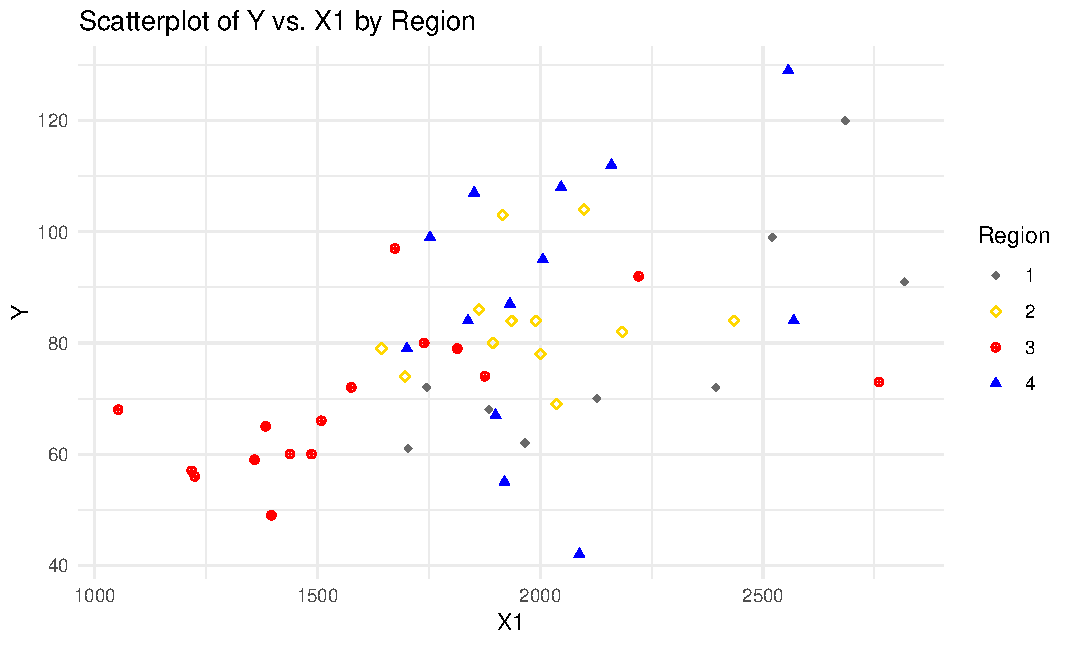
\includegraphics[width=.85\textwidth]{plot.symbols.colors_RJ.C.pdf}
           \end{enumerate} 
               % Complete the question about Y/X1

\end{itemize}


\end{document}
